% !TEX root = ../EjsS Manual.tex

\chapter{Installing and running \Ejs}\label{chapter:EjsIntro}

\begin{quote}
Machines should work. People should think.  {\em Richard Hamming}
\end{quote}

This introductory chapter provides an overview of \Ejs\ (\ejs\ for short), the high-level modeling and authoring tool that we use to teach modeling and simulation. We first describe the installation process and the file structure of our program, and then run the \ejs\ console to get our first \ejs\ program on the screen. We describe how \Ejs\  supports different programming languages for the modelling process. Subsequent chapters in this document provide a step-by-step introduction to the different parts of the \ejs\ graphical user interface, as well as to the modelling process. We finally instruct you how to download existing models created with \ejs\ from our on-line digital libraries.

% ------------------------
  \section{About \Ejs}
% ------------------------

Computer modeling is intimately tied to computer simulation.  A model is a conceptual representation of a physical system and its properties and modeling is the process whereby we construct this representation. Computer modeling requires (1) a description and an analysis of the problem, (2) the identification of the variables and the algorithms, (3) the implementation on a specific hardware-software platform, (4) the execution of the implementation and analysis of the results, (5) refinement and generalization, and (6) the presentation of results.
A computer simulation is an implementation of a model that allows us to test the model under different
conditions with the objective of learning about the model's behavior.\index{Simulation}  The applicability of the
results of the simulation to those of the real (physical) system depends on how well the model describes
reality.\index{Simulation!Model} The process of devising more general and more accurate models is what science is
about.

The implementation of a model and the visualization of its output requires that we program a computer. Programming can
be fun, because it gives us complete control of every visual and numerical detail of the simulated world. But
programming is also a technical task that can intimidate. This technical barrier can, however, be
lowered if we use an appropriate tool. \Ejs\ is a modeling tool that has been designed to allow
scientists, not only computer scientists, to create simulations in different programming languages.~\footnote{Currently, \ejs\ supports the Java and Javascript programming languages.} \ejs\ simplifies this task, both from the
technical and from the conceptual point of view.

\ejs\ provides a simple yet powerful conceptual structure for building simulations. The tool offers a sequence of
workpanels which we use to implement the model and its graphical user interface. \ejs\ automates tasks such as
numerically solving ordinary differential equations, \index{ODE} and animation (using separate threads, if required). The low-level communication between the program and the end-user that takes place at run-time, including handling of mouse actions within the simulation's graphical interface, is
accomplished without low-level programming.

Obviously, part of the task still depends on us. You are responsible for providing a model for the phenomenon and for
designing and selecting an output view that shows the model's main features. These high-level tasks are more related to
science than to programming. You are encouraged to devote your time and energy studying the science, something that the
computer cannot do. The purpose of this document is to demonstrate that this computer modeling is not only possible for non-programmers, but
can be relatively easy, with the help of \Ejs.

% ------------------------
    \section{Installing and running the Software}\label{section:02Installation}\index{\Ejs!installing and running}
% ------------------------

Let us begin by installing \Ejs\  and running it. \ejs\ is a Java program that can be run under any operating system
that supports a Java Virtual Machine (VM). Because Java is designed to be platform independent, the \ejs\ user
interface on Mac OS X, Windows, and Linux look very much the same, though they may present small differences among them. (We display the Mac OS X interface in the figures of this document.)

If \Ejs\ is not installed in your computer, you need to do so now. To \textbf{install} \ejs, do the following:

\begin{numberlist}

\item \textbf{Install the Java Runtime Environment.} \ejs\ requires the Java Runtime Environment (JRE), \textbf{version 1.7 or later}.
The JRE may already be installed in your computer, but, if not, visit the Java site at \link{http://java.com} and follow the instructions there
to download and install the latest version.

\item \textbf{Copy the \ejs\ distribution file to your computer.} \ejs\ is distributed in a compressed ZIP file that can be downloaded from \ejs\ web site \link{http://www.um.es/fem/EjsWiki}. The distribution file will be called something like \file{EjsS\_X.x\_yymmdd.zip}. 
Here, the \texttt{X.x} characters stand for the actual version of the software, and \texttt{yymmdd} stands for the date this version was created. (For instance, you can get something like \file{EjsS\_5.2\_161123.zip}.)

\item \textbf{Uncompress \ejs.} Uncompress the \ejs\ distribution file on your computer's hard disk to create a directory called \file{EjsS\_X.x} (\file{EjsS\_5.2} in the example). The new directory contains the whole \ejs\ program.
\note{In Unix-like systems, the \file{EJS\_X.x} directory may be uncompressed as read-only. Enable write
permissions for the \file{EjsS\_X.x} directory and all its subdirectories.}
\end{numberlist}

And that's it! This is all that is needed to install \ejs. Once \Ejs\ is installed in your computer, do the following to \textbf{run} \ejs:

\begin{description}
\item \textbf{Run the \ejs\ console.} Inside the newly-created \file{EJS\_X.x} directory, you will find a file called
\file{EjsConsole.jar}.\index{jar files!EjsConsole.jar}\index{Easy Java Simulations!console} Double-click it to run the
\ejs\ console shown in Figure~\ref{fig:01Introduction/EjsConsole}.
\note{If double-clicking doesn't run the console, open a
system terminal window, change to the \file{EJS\_X.x} directory, and type the command: \code{java -jar EjsConsole.jar}.
You'll need to fully qualify the \code{java} command if it is not in your system's PATH.}
\end{description}

\begin{figure}[htb]
  \centering
%  \subfigure[Console's basic options tab.]{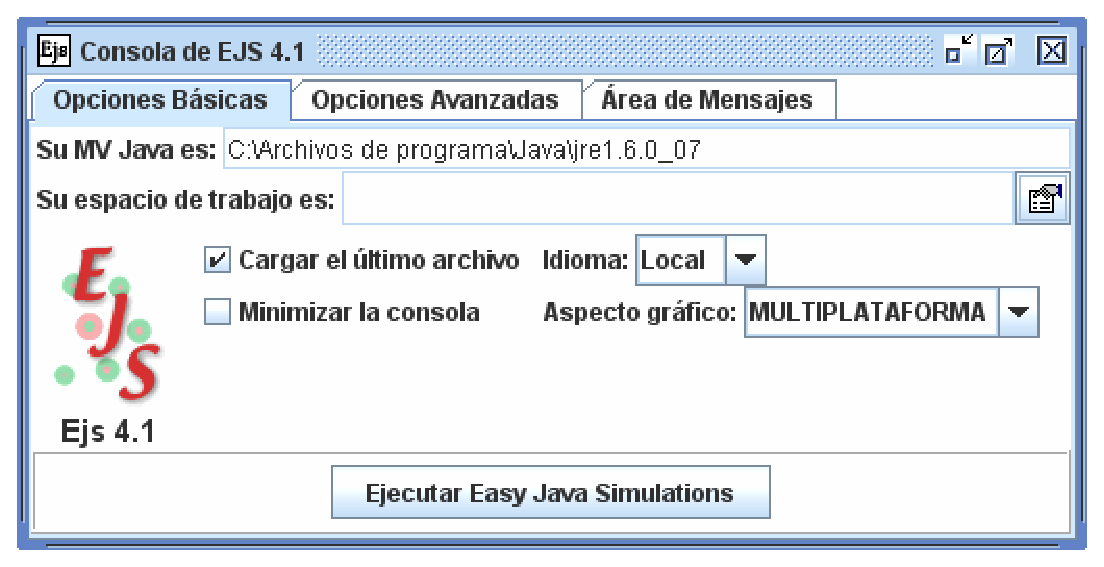
\includegraphics[scale=\scale]{01Introduction/images/EjsConsole1.eps}}
%  \subfigure[Console's output area.]{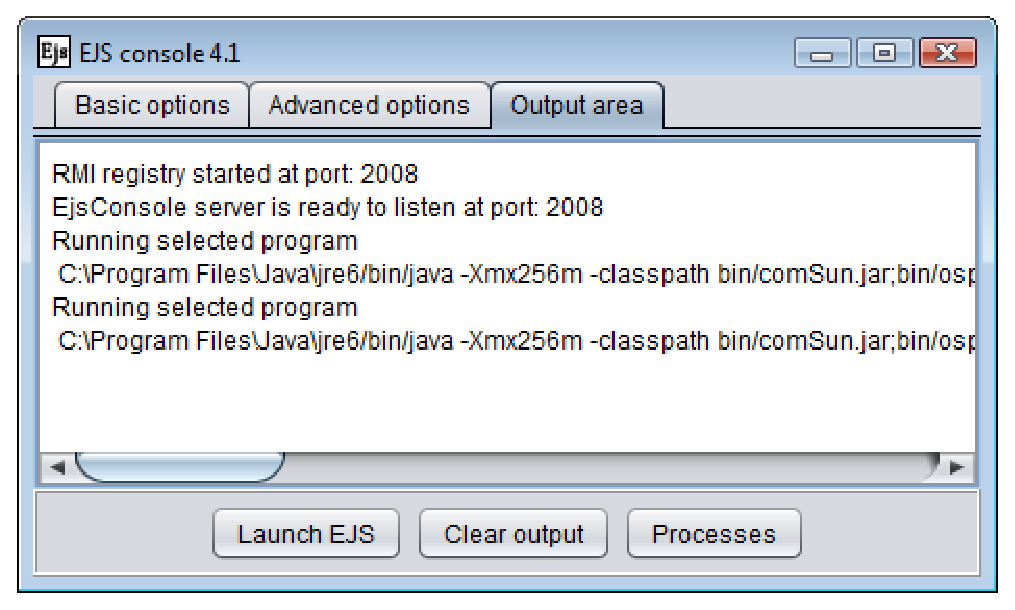
\includegraphics[scale=\scale]{01Introduction/images/EjsConsole2.eps}}
%  \caption{Two views of the \ejs\ console.}
  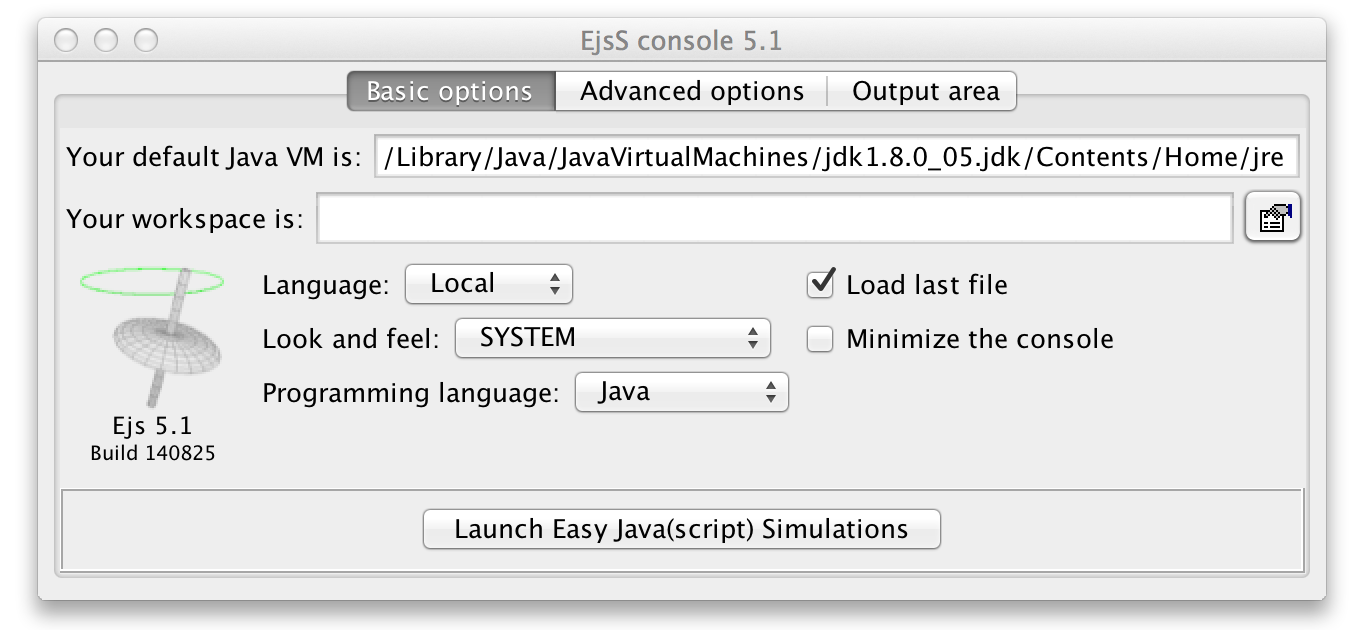
\includegraphics[scale=\scale]{01Introduction/images/EjsConsole1.png}
  \caption{The \ejs\ console.}
  \label{fig:01Introduction/EjsConsole}
\end{figure}

You should see the console (Figure~\ref{fig:01Introduction/EjsConsole}) and the file chooser dialog of Figure~\ref{fig:01Introduction/WorkspaceChooser}, that we will describe below, on your computer display.

\begin{figure}[htb]
  \centering
  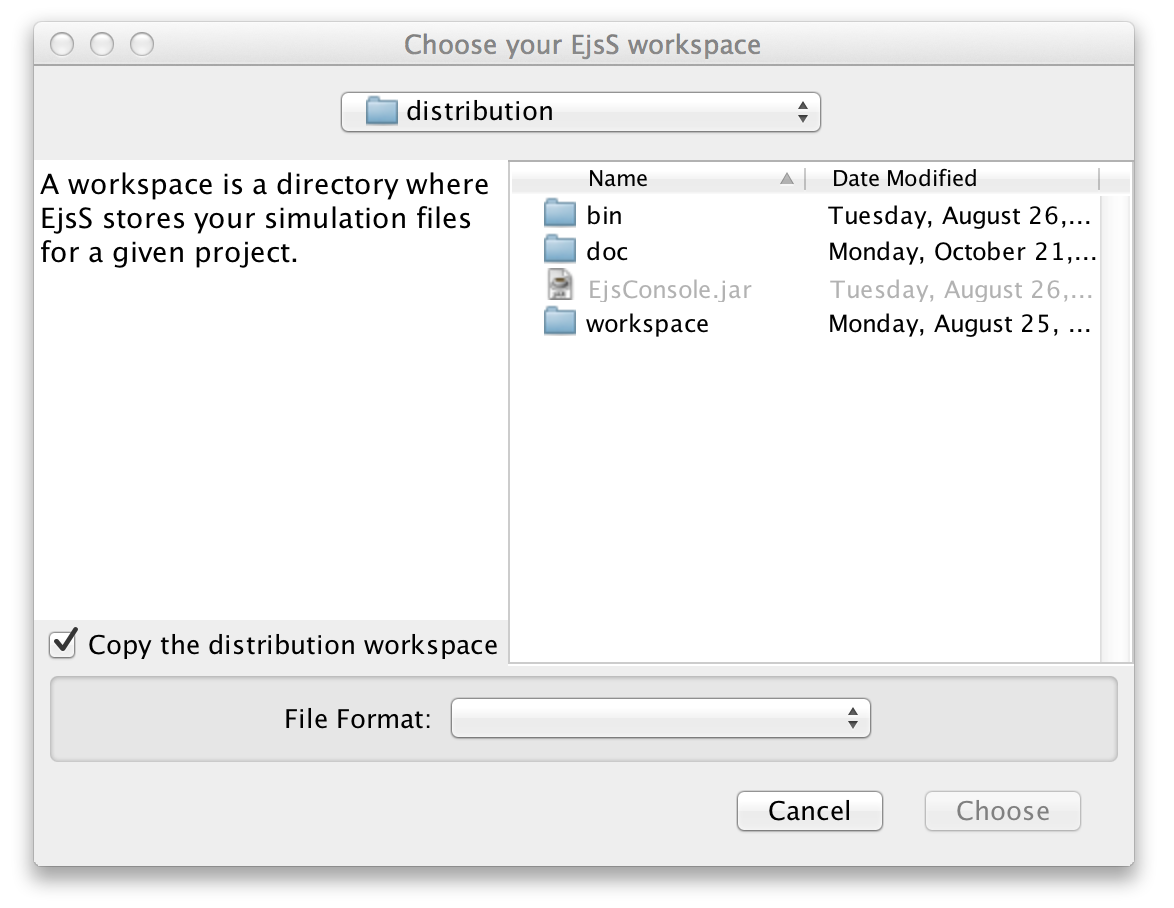
\includegraphics[scale=\scale]{01Introduction/images/WorkspaceChooser.png}
  \caption{File chooser to select your workspace directory.}
  \label{fig:01Introduction/WorkspaceChooser}
\end{figure}

The \ejs\ console is not part of \ejs, but a utility used to launch one or several instances (copies) of \ejs\ and to perform other \ejs-related tasks. You can use the console to customize some aspects of how \ejs\ looks and behaves at start up.~\footnote{For instance, set the \lit{Look and feel} field to \lit{CROSS\_PLATFORM}, the specific look and feel identical across all platforms, and launch a new instance of \ejs\ to apply the change. We set the default look and feel to \lit{SYSTEM}, the default for your platform. The one shown in this document corresponds to the characteristic \lit{Aqua} look an feel of Mac OS X.} The console also displays \ejs\ program information and error messages on its \lit{Output area} tab, and we will refer to it from time to time in this document. The console creates an instance of \ejs\ at start-up and exits automatically when you close the last running instance of \ejs. 
%Other console features, such as its ability to process collections of \ejs\ models, are described in the appendices.

However, before the console can run \ejs\ right after installation, the file chooser displayed in Figure~\ref{fig:01Introduction/WorkspaceChooser} will appear, letting you select the directory in the computer hard disk that you will use as your \emph{workspace}.
\ejs\ uses the concept of a workspace to organize your work. A workspace is a directory in your hard disk where \ejs\ stores your simulation files for a given project. A workspace can contain an unlimited number of simulations. Inside a workspace directory, \ejs\ creates four subdirectories:\index{\Ejs!directory structure}
\begin{bulletlist}
  \item \file{config} is the directory for user-defined configuration and options files.
  \item \file{export} is the proposed target directory when \ejs\ generates files for distribution.
  \item \file{output} is the directory used by \ejs\ to place temporary files generated when compiling a simulation.
  \item \file{source} is the directory under which all your simulation (source and auxiliary) files must be located.
\end{bulletlist}

When you first run \ejs, the console asks you to choose a workspace directory. This must be a writable directory anywhere in your hard disk. You can choose to use the workspace included in the distribution, i.e. the \file{workspace} directory in the \file{EJS\_X.x} directory created when you unzipped the \ejs\ bundle. But it is \textbf{highly recommended} to create a new directory in your usual personal directory (or, better yet, in a cloud-accesible directory --- like \lit{Dropbox} \link{http://dropbox.com}, or similar). The file dialog that allows you to choose the workspace has a check box that, when checked, will copy all the examples files of the distribution to the new workspace. Leave this check box checked and you will find some subdirectories in the \file{source} directory of your workspace which contain sample simulations. In particular, you will find the \file{JavaExamples} and \file{JavascriptExamples} directories described in later chapters of this document.

\note{Although generally not needed, you can create and use more than one workspace for different projects or tasks. The console provides a selector to let you change the workspace in use and \ejs\ will remember the current workspace between sessions or even if you reinstall \ejs.}

Finally, the first time you run \ejs, the program will also ask you to introduce your name and affiliation (Figure~\ref{fig:01Introduction/NameAndAffiliation}). This step is optional but recommended, since it will help you document your future simulations. You can choose to input or modify this information later using the options icon of \ejs' task bar.

\begin{figure}[htb]
  \centering
  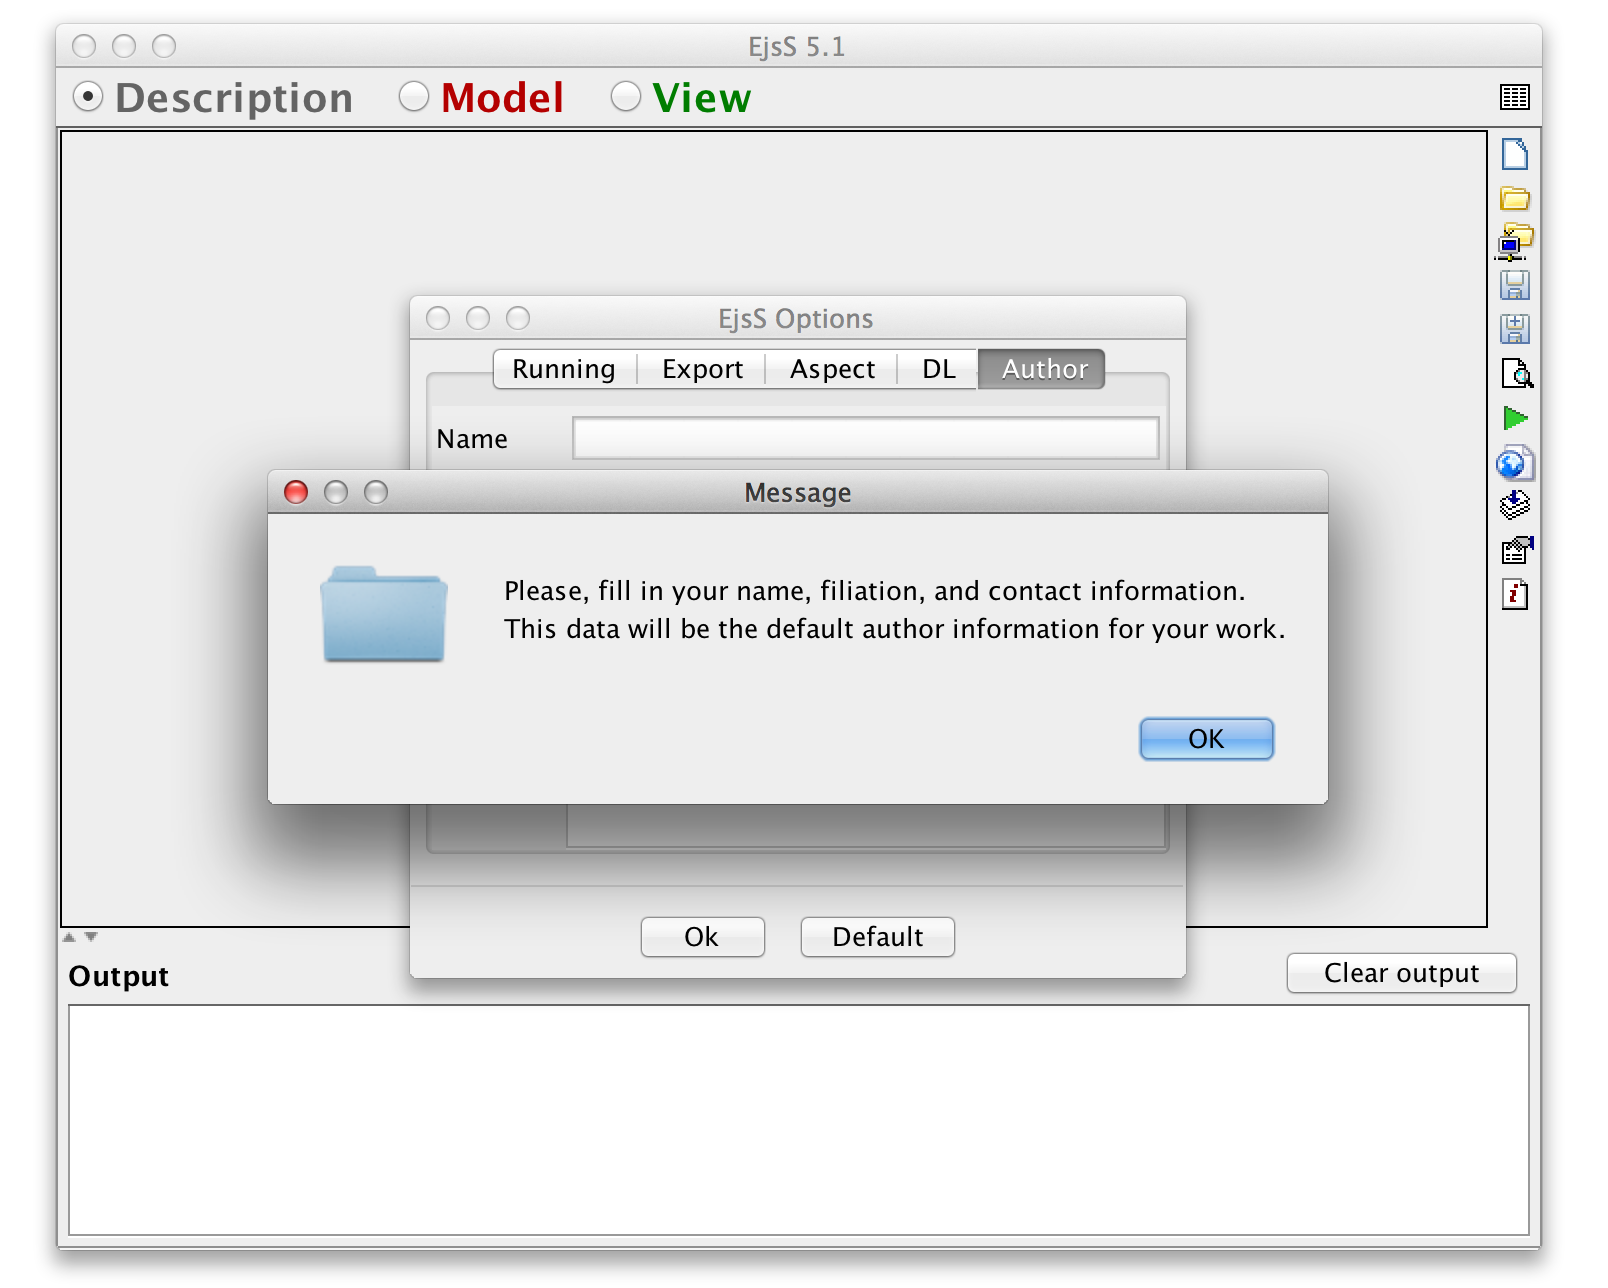
\includegraphics[scale=\scale]{01Introduction/images/NameAndAffiliation.png}
  \caption{Optionally input your name and affiliation.}
  \label{fig:01Introduction/NameAndAffiliation}
\end{figure}

% ------------------------
    \section{The graphical user interface}\label{section:01GUI}\index{\Ejs!graphical user interface}
% ------------------------

We are now ready to turn our attention to the \ejs\ modeling tool, displayed with annotations in
Figure~\ref{fig:01Introduction/EjsInterface}. Despite its simple interface, \ejs\ has all the tools needed for a complete
modeling cycle.

\begin{figure}[htb]
  \centering
  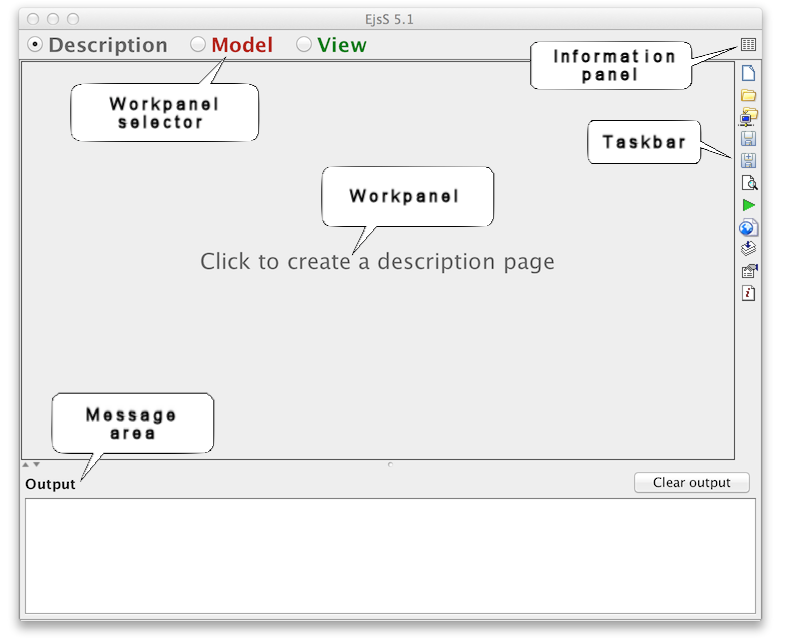
\includegraphics[scale=\scale]{01Introduction/images/EjsInterface.png}
  \caption{The \Ejs\ user interface with annotations.}
  \label{fig:01Introduction/EjsInterface}
\end{figure}

The taskbar\index{\Ejs!taskbar} on the right provides a series of icons to
clear, open, search, and save a file, configure \ejs, and display program information and help. It also provides icons to run a
simulation and to package one or more simulations in a self-contained file. Right-clicking on taskbar icons invokes alternative (but related) actions that will be described as needed. The bottom part of the interface contains an output area\index{\Ejs!output area} where \ejs\ displays informational messages. The central part of the interface contains the workpanels where the modeling is done.

\Ejs\ provides three workpanels for modeling. The first panel, \lit{Description}, allows us to create and edit
multimedia HTML-based narrative that describes the model.\index{HTML} Each narrative page appears in a tabbed panel
within the workpanel and right-clicking on the tab allows the user to edit the narrative or to import additional
narrative. The second work panel, \lit{Model}, is dedicated to the modeling process. We use this panel to create
variables that describe the model, to initialize these variables, and to write algorithms that describe how this model
changes in time. The third workpanel, \lit{View} or \lit{HtmlView} (for HTML5-based interfaces), is dedicated to the task of building the graphical user interface,
which allows users to control the simulation and to display its output. We build the interface by selecting elements
from palettes and adding them to the view's \lit{Tree of elements}. For example, the \lit{Interface} palette contains
buttons, sliders, and input fields and the \lit{2D Drawables} palette contains elements to plot 2D data.

% ------------------------
   % \subsection{Programming languages support}\label{section:02Languages}\index{\Ejs!programming languages}
% ------------------------

\Ejs\ supports more than one programming languages to implement the algorithms required for the modeling process. The interface of all of them is based on the same principles, and learning to use one of them, leads to understanding them all. We sometimes refer to the different interfaces of \Ejs\ for the different programming languages, as the \emph{flavors} of \ejs. Hence, we may refer to the \emph{Java flavor} or the \emph{Javascript flavor} of \ejs, for instance.

The \ejs\ console launches, by default, an instance of \ejs\ which supports the Java programming language (i.e. an instance of the Java flavor of \ejs). You can change the supported programming language or flavor (using the \lit{Programming language} selector in the \lit{Basic} tab of the \ejs\ console), and launch another instance of \ejs\ for this language clicking the \lit{Launch \ejs} button. Figure~\ref{fig:01Introduction/EjsInterfaceJS} displays the graphical user interface for the creation of Javascript models in \Ejs.

\begin{figure}[htb]
  \centering
  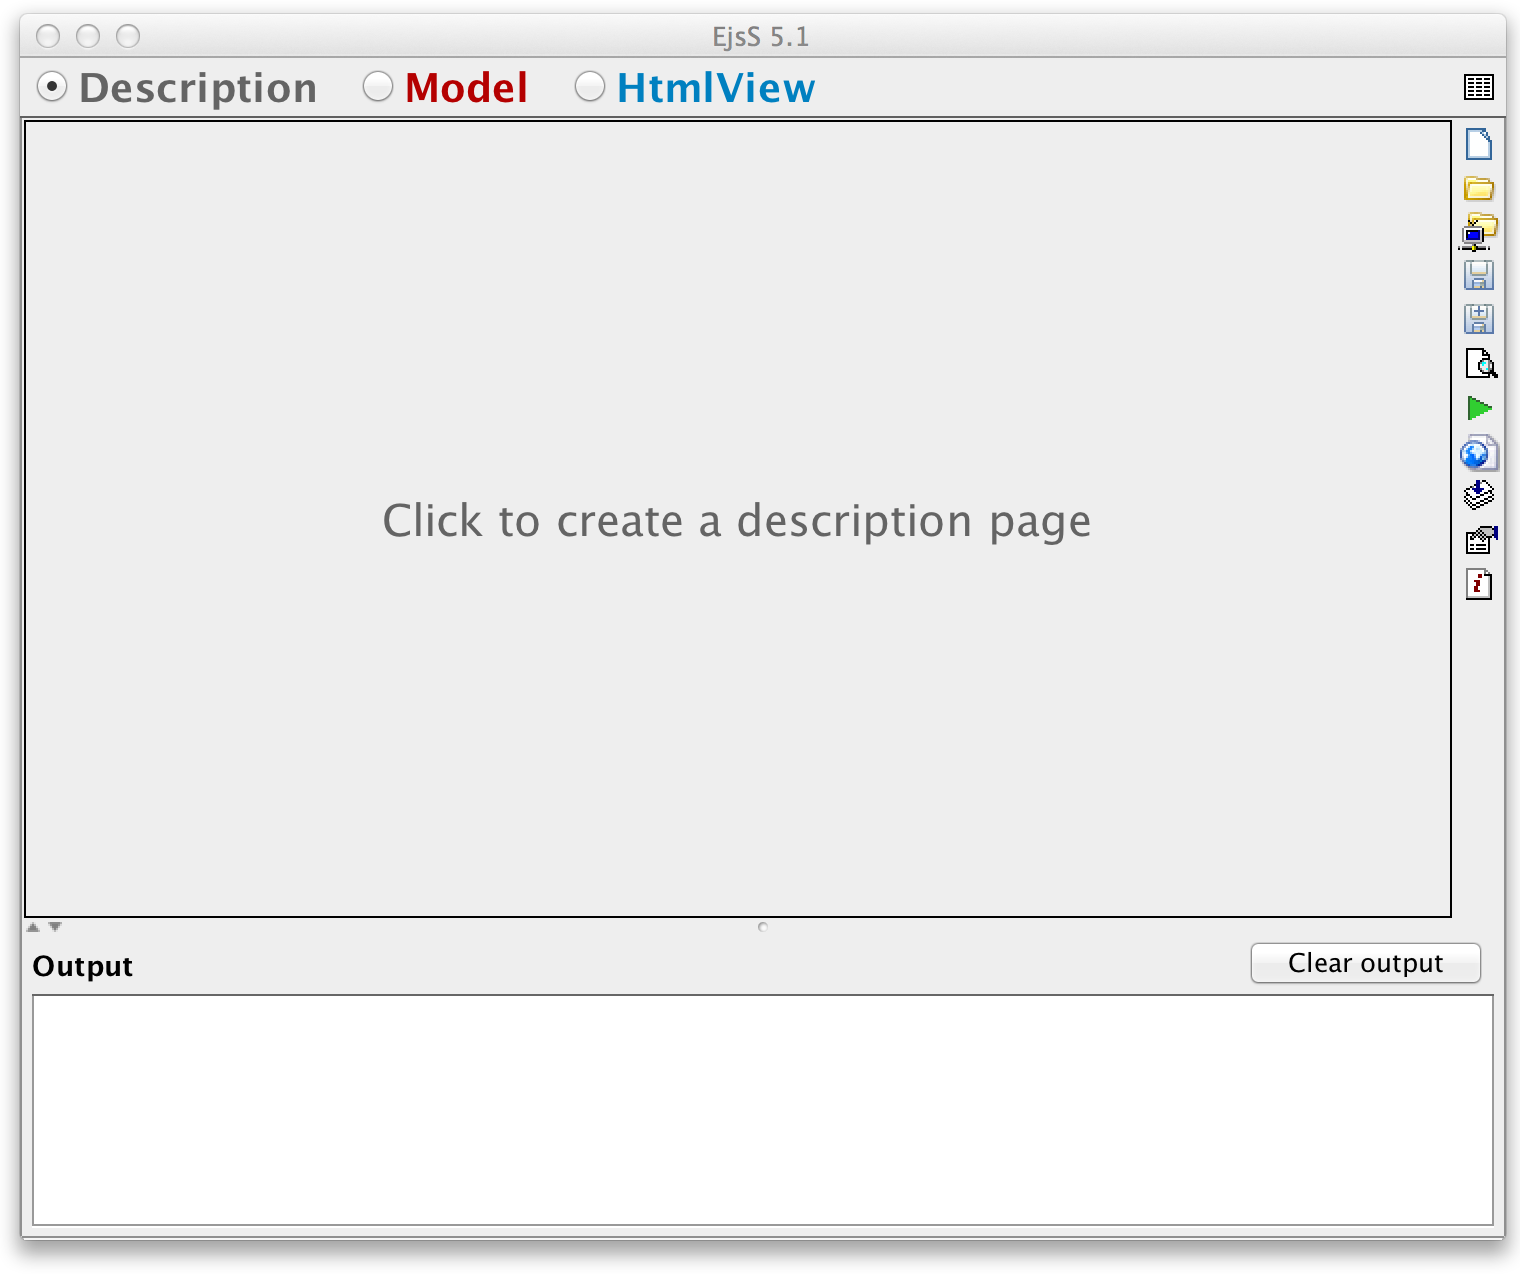
\includegraphics[scale=\scale]{01Introduction/images/EjsInterfaceJS.png}
  \caption{The \Ejs\ user interface for Javascript support.}
  \label{fig:01Introduction/EjsInterfaceJS}
\end{figure}

The next two chapters of this document guide you to inspect in detail and run an already existing simulation in each of the supported programming languages. (The simulation models the same physical phenomenon in all cases.) This will help you understand how the \lit{Description}, \lit{Model}, and \lit{View} (or \lit{HtmlView}) workpanels work together to help you model a simulation. 
If you are new to \Ejs, please read the chapter for the \ejs\ flavour you are most interested in before exploring any of the many existing models in our digital libraries.

% -----------------------------------------------------
\section{Finding models}\label{section:01FindingModels}
% -----------------------------------------------------

Once you have covered the basics of \ejs\ and you know how to load, inspect, run, and even modify an example, you may be interested in finding existing simulations to see what  other users have done with \ejs. Maybe, you can find a model that already fits your needs or that you can easily modify to be ready for classroom use.

There are two places you can look at to find more models.
The first place to look at is the source sample directory that came with your distribution of \ejs. In the source directory of the distribution's workspace you will find some directories with sample simulations. These sample directories were also copied to your own workspace (unless you unselected this option) when you first run \ejs.

The second, and perhaps more interesting, place (actually places) to look for new models are available through the Internet. The \ejs\ digital libraries icon in the taskbar, 
\includegraphics[scale=\linescale]{../_common/icons_png/netOpen.png}, opens a window which allows you to connect to repositories of \ejs\ models available through the Internet. This window, displayed in Figure~\ref{fig:01Introduction/EJSDigitalLibraries}, contains a combo box at its top that lists the available digital libraries. A second combo box lets you select the desired programming language for the models.  Select one of these libraries, the programming language, or click the \lit{Refresh} button to get the list of \ejs\ models in it. All these libraries work in a similar way, and we use the \textbf{comPADRE} digital library repository to illustrate how they are accessed from within \ejs.

\begin{figure}[htb]
    \centering
  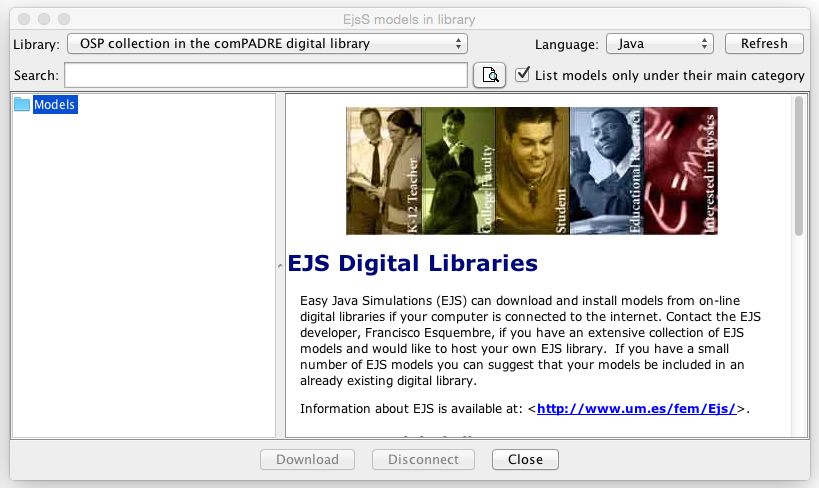
\includegraphics[scale=\scale]{01Introduction/images/EJSDigitalLibraries.png}
    \caption{The Digital Libraries window of \ejs. Select one of the available repositories using the combo box at the top of the window, the preferred programming language, or click the \lit{Refresh} button to retrieve the list of models available.}
    \label{fig:01Introduction/EJSDigitalLibraries}
\end{figure}

The \textbf{comPADRE Pathway}, a part of the (USA) National Science Digital Library, is a growing network of educational resource collections supporting teachers and students in Physics and Astronomy. Of special relevance for our interests is the Open Source Physics comPADRE collection available at \link{http://www.compadre.org/OSP}. This collection contains computational resources for teaching in the form of executable simulations and curriculum resources that engage students in physics, computation, and computer modeling. In particular, it contains \ejs\ models whose source (XML) code can be accessed directly from \ejs\ using the digital libraries icon.

If you are connected to the Internet, select the \lit{OSP collection on the comPADRE digital library} entry of the top combo box and \ejs\ will connect to the library to obtain the very latest catalog of \ejs\ models in the library. At the moment of this writing, there are some 500 Java models and  200 Javascript models organized in different categories and subcategories, and the collection is expected to grow. As the left frame of Figure~\ref{fig:01Introduction/OSPCollection} shows, the collection is organized in categories and subcategories. When the name of a subcategory appears in red, double-click it to expand the node with the list of models of the subcategory. Because many models have primary and secondary classifications, a check box at the top pane, next to the \lit{Search} field, allows you to decide whether you want the models to be listed uniquely under their primary classification, or appear in all matching categories (thus appearing more than once).

\begin{figure}[htb]
    \centering
  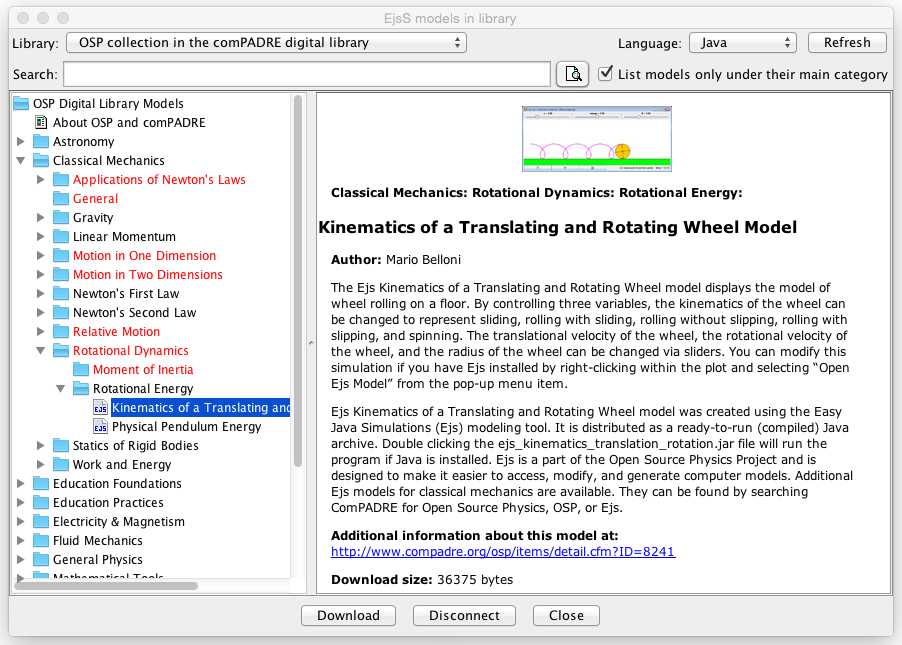
\includegraphics[scale=\scale]{01Introduction/images/OSPCollection.png}
    \caption{The OSP collection on the comPADRE digital library. The collection is organized in categories and subcategories. The entry for a model provides information about the model.}
    \label{fig:01Introduction/OSPCollection}
\end{figure}

When you click a model node, the right frame shows information about the model obtained instantly from the library. The information describes the model, and includes a direct link to the comPADRE library for further information. Double-clicking the model entry, or clicking the \lit{Download} button, will retrieve the model and auxiliary files from the library, ask you for a place in your source directory of your workspace to download them, and open the model in \ejs\ when the download is complete. Because source files are usually small, the download takes place almost instantly. Now, you can inspect, run, or modify the model as shown in the exploration chapters below, for the mass and spring model.

The OSP collection on the comPADRE digital library is a highly recommended place to look for \ejs\ models and accompanying curricular material. 
%We will often include references to models in the comPADRE digital library in this document, whenever they relate to the narrative.

% -----------------------------------------------------
\section{Summary}\label{section:02Review}
% -----------------------------------------------------

\Ejs\ is a modeling and authoring tool expressly devoted to the task of creating computer simulations to study and display a wide range
of phenomena ranging from the simple to the complex. These computer simulations are used to obtain numerical data from our models as they advance in time, and to display this data in a form humans can understand.

\ejs\ has been designed to let us work at a high
conceptual level, concentrating most of our time on the scientific aspects of our simulation, and asking the computer
to automatically perform all the other necessary but easily automated tasks.
%\ejs\ structures the authoring process in three parts: creating a description, specifying the model, and building the view for the simulation. Each task has a dedicated workpanel that provides the needed functionality. The description workpanel is used to create a set of multimedia HTML pages which provide the necessary narrative to put the model into context. These pages are displayed from within \ejs\ itself, but also when we distribute the simulation in form of a Java applet or within a Launcher package. Creating the model is one of our main tasks, and \ejs\ organizes the process by providing a series of panels that we edit, left to right, to complete the specification: declaration and initialization of variables, evolution pages, constraints (fixed relationships among variables), and custom code. Each panel has specialized capabilities.  The ODE editor stands out and we will see how advanced this editor is when we model many-particle ensembles with arrays. Finally, building the view is made easier by the use of off-the-shelf, ready to use view elements, of which there are many different types, each one specialized for a given visualization or input task. These elements have properties that can be edited to give them either constant or dynamic values that change according to the evolution of the model. We can use these elements to build views whose effectiveness and sophistication rival the work of a professional programmer. Once this high-level work is done, a single mouse click starts the internal engine that will generate a fully dynamic, interactive simulation from our specifications.
Every tool, including \Ejs, has a learning curve. The rest of this document contains a series of detailed examples that will familiarize you with the modeling, visualization, and interaction capabilities of \ejs. 
%The second part of the document  is devoted to advanced examples, and emphasizes the scientific content of the models and their behavior. 
%The appendices cover additional features such as a porting a simulation across programming languages. 
%review of Java and guidelines that will help you through the unavoidable moment when you make your first programming mistakes.

Modeling is both a science and an art. \Ejs\ is a tool that lets you express your science knowledge by facilitating the techniques required by the art, and by providing simple access to many modeling examples from other authors.





